\documentclass[a4paper,english]{lipics-v2019}
\usepackage{wrapfig,microtype,amssymb,amsmath,stmaryrd,mathpartir,array,graphicx,tabularx,xspace}
\usepackage[table]{xcolor}
\newcommand{\xt}[1]{\texttt{#1}}
%\newcommand{\tupleo}[1]{\xt{Tuple1\{}#1\xt{\}}}
\newcommand{\tuplet}[2]{\xt{Tuple\{}#1,#2\xt{\}}}
\newcommand{\union}[2]{\xt{Union\{}#1,#2\xt{\}}}
\newcommand{\denotes}[1]{\llbracket #1 \rrbracket}

\renewcommand{\L}{{\tt L}\xspace}
\newcommand{\Ls}{{\tt L}s\xspace}
\newcommand{\R}{{\tt R}\xspace}
\newcommand{\uL}{{\underline{\tt L}}\xspace}
\renewcommand{\c}[1]{\lstinline{#1}\xspace}

%FZ
\newcommand{\sub}{<:}
\newcommand{\tuple}[1]{\xt{Tuple\{}#1\xt{\}}}
\newcommand{\arrayt}[1]{\xt{Array\{}#1\xt{\}}}
\newcommand{\FZ}[1]{\textbf{FZ says: #1}}
%end FZ

\newcommand{\goodcell}{\cellcolor{green!25}}
\newcommand{\badcell}{\cellcolor{red!25}}
\bibliographystyle{plainurl}% the recommnded bibstyle
\title{Julia's efficient algorithm for subtyping unions and covariant tuples}
\titlerunning{Subtyping union types and covariant tuples}

\author{Benjamin Chung}{Northeastern University}{}{}{}%mandato
\author{Francesco Zappa Nardelli}{INRIA}{}{}{} \author{Jan
  Vitek}{Northeastern University \& Czech Technical University in
 Prague}{}{}{}
\authorrunning{B. Chung, F. Zappa Nardelli, J. Vitek}
\Copyright{Benjamin Chung, Francesco Zappa Nardelli, Jan Vitek}%mandatory, plea
\ccsdesc[500]{Theory of computation~Type theory}
\keywords{Type systems, Subtyping, Union types}

\lstset{
 language=caml,
 columns=[c]fixed,
 basicstyle=\small\ttfamily,
 keywordstyle=\bfseries,
 upquote=true,
 commentstyle=,
 breaklines=true,
 showstringspaces=false}

%Editor-only macros:: begin (do not touch as author)%%%%%%%%%%%%%%%%%%%%%%%%%%%%%%%%%%
\EventEditors{John Q. Open and Joan R. Access}
\EventNoEds{2}
\EventLongTitle{42nd Conference on Very Important Topics (CVIT 2016)}
\EventShortTitle{ECOOP}
\EventAcronym{ECOOP}
\EventYear{2019}
\EventDate{December 24--27, 2016}
\EventLocation{Little Whinging, United Kingdom}
\EventLogo{}
\SeriesVolume{42}
\ArticleNo{23}
%%%%%%%%%%%%%%%%%%%%%%%%%%%%%%%%%%%%%%%%%%%%%%%%%%%%%%

\begin{document}

\maketitle
\begin{abstract}
  The Julia programming language supports multiple dispatch and provides a
  rich type annotation language to specify method applicability. When
  multiple methods are applicable for a given call, Julia relies on
  subtyping between method signatures to pick the method to invoke. Julia's
  subtyping algorithm is surprisingly complex, and deciding whether it is
  correct remains an open question. In this paper, we focus on a piece of
  the problem, the interaction between union types and covariant
  tuples. Previous work that addressed this particular combination of
  features did so by normalizing types to a disjunctive normal form
  ahead-of-time. Normalization is not practical due to space-explosion for
  complex type signatures and to interactions with other features of Julia's
  type system.  Our contribution is a description of the algorithm
  implemented in the Julia run-time system. This algorithm is immune to the
  space-explosion and expressiveness problems of standard algorithms.  We
  prove this algorithm correct and complete against a semantic-subtyping
  denotational model in Coq.
\end{abstract}

\section{Introduction}

Union types, originally introduced by Barbanera and
Dezani-Ciancaglini~\cite{barbanera1991intersection}, are increasingly being
used in mainstream languages. In some cases, as Julia~\cite{BezansonEKS17}
or TypeScript~\cite{typescript}, they are exposed at the source level. In
others, such as Hack~\cite{hack}, they are only used internally when
performing type inference. We describe a space-efficient technique for
computing subtyping between types in the presence of distributive unions.
Our motivation arises from the Julia programming language. In our previous
work on formalizing the Julia subtyping
algorithm~\cite{DBLP:NardelliBPCBV18}, we described the subtyping relation
but were unable to describe the subtyping algorithm or prove it
correct. Indeed, we found bugs and were left with unresolved issues.

Julia's subtyping algorithm is an important part of its semantics. Julia is
a dynamically typed language where methods are annotated with type
signatures to enable multiple dispatch. During program execution, Julia must
determine which method to invoke at each call site. It does so by finding
the most specific applicable method (according to subtyping) that applies
for a given invocation. The following snippet shows three declarations of
multiplication.

\begin{lstlisting}
 *(x::Number, r::Range)  = range(x*first(r),...)
 *(x::Number, y::Number) = *(promote(x,y)...)
 *(x::T, y::T) where T <: Union{Signed,Unsigned} =  mul_int(x,y)
\end{lstlisting}

\noindent The first two methods implement, respectively, the case where a
range is multiplied by a number and generic numeric multiplication. The
third method invokes native multiplication when both arguments are either
signed or unsinged integers (but not a mix of the two).

Julia offers programmers a rich type language, including nominal single
subtyping, union types, existential types, covariant tuples, invariant
parametric datatypes, and singleton types. These features are widely used in
libraries, but pose challenges for subtyping. The design of subtyping was
inspired by semantic subtyping~\cite{Frisch02,BezansonEKS17}, but Julia
departs from that intuitive understanding of  the meaning of types.

This paper documents the first steps towards proving the correctness of
Julia's subtyping algorithm. We focus on the interaction of two features:
union types and covariant tuples. Tuples are used to represent function
signatures (Julia does not record return types). They are covariant as a
function with more specific arguments is preferred to a more generic one.
Union types are used as shorthand to avoid having to write multiple
functions with the same body.  Rules for subtyping union types and covariant
tuples have been known for a long time. Based on Vouillon~\cite{Vouillon04},
the following is a typical deductive system:

\vspace{-3mm}{\small\begin{mathpar}
\inferrule[allexist]{
   t' \sub t \\ t'' \sub t}{\union{t'}{t''} \sub t}

\inferrule[existL]{t \sub t'}{t \sub \union{t'}{t''}}

\inferrule[existR]{t \sub t''}{t \sub \union{t'}{t''}}

\inferrule[tuple]{t_1 \sub t'_1 \\ t_2 \sub t'_2}{\tuple{t_1, t_2} \sub \tuple{t'_1, t'_2}}
\end{mathpar}}
\vspace{-3mm}

\noindent While this rule system makes sense, it does not match the
intuition for subtyping. If we think of types as sets of
values~\cite{Pierce1991}, we would expect that a union type would be
analogous to set theoretic union. Similarly, we would then expect that two
types would be subtypes if their sets of values were subsets.  Therefore,
when a union type appears on the left-hand side of a judgment, \emph{all}
its components must be subtypes of the right-hand side; when a union type
appears on the right-hand side of a judgment, there must \emph{exist} a
component that is a supertype of the left-hand side. The above
system of rules violates these ideas. Consider the following judgment:

%
\vspace{-3mm}{\small\[
\tuple{\union{t'}{t''}, t} \ \ \sub\ \ \union{\tuple{t', t}}{\tuple{t'', t}} 
\]}
\vspace{-3mm}
%

\noindent Under a semantic subtyping, the judgment should hold. We write the
set of values denoted by the type $t$ as {\small $\llbracket t \rrbracket$}.
The left hand side denotes the values {\small $\{\tuple{v',v''} ~|~ v' \in
  \llbracket t' \rrbracket \cup \llbracket t'' \rrbracket \wedge v'' \in
  \llbracket t \rrbracket\}$}, while the right hand side denotes {\small
  $\llbracket \tuple{t', t} \rrbracket \cup \llbracket \tuple{t'', t}
  \rrbracket$}.  Obviously, the sets are the same. However, we cannot derive
this relation from the above rules. According to them, we must pick either
{\small $t'$} or {\small $t''$}, ending up with either {\small
  $\tuple{\union{t'}{t''}, t} \sub \tuple{t', t}$} or {\small
  $\tuple{\union{t'}{t''}, t} \sub \tuple{t'', t}$}. In either case, the
judgment does not hold.

Some early work~\cite{barbanera1991intersection,Pierce1991} uses
normalization to decide distributive subtyping between union types, while
Vouillon~\cite{Vouillon04} does not handle distributivity. Normalization
entails rewriting all types into their disjunctive normal form, as unions of
union-free types, \emph{before} building the derivation. This lifts all
choices to the top level, avoiding the structural entanglements that cause
trouble. The correctness of this rewriting step is justified by the
semantic-subtyping denotational model~\cite{Frisch08}, and the resulting
subtype algorithm can be proved both correct and complete. However, this
algorithm has two major drawbacks: it is not space efficient and it does not
interact well with other features of Julia..

The first drawback is that the normalization can lead to exponentially
bigger types. Real-world Julia code has types like the
following~\cite{DBLP:NardelliBPCBV18} whose normal form has 32,768
constituent base types, making it impractical to store or to compute with:


\begin{small}
\begin{verbatim}
 Tuple{Tuple{Union{Int64, Bool}, Union{String, Bool}, Union{String, Bool}, 
             Union{String, Bool}, Union{Int64, Bool}, Union{String, Bool}, 
             Union{String, Bool}, Union{String, Bool}, Union{String, Bool}, 
             Union{String, Bool}, Union{String, Bool}, Union{String, Bool}, 
             Union{String, Bool}, Union{String, Bool}, Union{String, Bool}}, Int64}
\end{verbatim}
\end{small}

The second drawback of normalisation is that it does not interact well with
other features of the type system. For instance, Julia supports invariant
constructors, which are incompatible with union normalization. For example,
the type $\arrayt{\xt{Int}}$ is an array of integers, this type is not be a
subtype of $\arrayt{\xt{Any}}$. This seemingly simple feature, in
conjunction with type variables, makes normalization ineffective.
Consider the type {\small \(\arrayt{\union{t'}{t''}}\)}. This type denotes the set
of arrays whose elements are either of type {\small $t'$} or {\small   $t''$}.
It would be incorrect to rewrite it as {\small
\(\union{\arrayt{t'}}{\arrayt{t''}}\)}, as this latter type denotes the set of
arrays whose elements are either all of type {\small $t'$} or all of type
{\small$t''$}. A weaker disjunctive normal form, only lifting union types
inside each invariant constructor, can circumvent this problem. However, doing
so only to reveals a deeper problem in thfe presence of both invariant
constructors and {existential types}. This is illustrated by the following judgment:

%
\vspace{-3mm}{\small\[
  \arrayt{\union{\tuple{t}}{\tuple{t'}}} \ \ <:\ \ \exists T\,.\, \arrayt{\tuple{T}}
\]}\vspace{-3mm}
%

\noindent 
This judgment holds if we set the existential {\small$T=\union{t}{t'}$}.
Since all types are in weak normal form, an algorithm based on the standard
system of judgment rules would strip off the array type constructors and
proceed.  However, since type constructors are invariant on their arguments,
it must first test that the relation holds in the original order (e.g. that
$\union{\tuple{t}}{\tuple{t}} <: \tuple{T}$) and in the reverse order (that
$\tuple{T} <: \union{\tuple{t}}{\tuple{t'}}$). It is in this combined check
that we run into problems.
%
The original order subtype check can be concluded without issue, producing
the constraint on $T$ {\small$\union{t}{t'} <: T$}. However, this constraint
on $T$ is stored for checking the reversed direction of subtyping, which is
where the problems arise. When we check the opposite subtype order, we end
up having to prove that {\small$\tuple{T}<:\union{\tuple{t}}{\tuple{t'}}$}
and in turn either {\small$T<:t$} or {\small$T<:t'$}. All of these are
unprovable under the assumption that {\small$\union{t}{t'} <: T$}.
%
The key to derive a successful judgment for this relation is to rewrite the
right-to-left check into {\small$\tuple{T}<:\tuple{\union{t}{t'}}$}, which is
provable. This \emph{anti-normalisation} rewriting must be performed on
sub-judgments of the derivation, and to the best of our knowledge it is not
part of any subtype algorithm based on ahead-of-time disjunctive
normalisation. As a result, straightforward normalization, even to a relaxed
normal form, is incompatible with the full Julia type system.

In this paper we describe the key ideas used by the subtype algorithm
implemented in the Julia language to deal with union types and covariant
tuples. This strategy avoids both aforementioned problems, though we will
focus  on the way that it solves the space explosion issue. To avoid being
drawn in the vast complexity of Julia type algebra, we focus on a minimal
language featuring union types, covariant tuples, and literals. This tiny
language is expressive enough to highlight the decision strategy, and make
this implementation technique known to a wider audience.  While Julia
implementation shows that this technique extends, among others, to invariant
constructors and existential types~\cite{DBLP:NardelliBPCBV18}, we expect that
it can be leveraged in many other modern language designs. Additionally we
prove in Coq that the algorithm is correct and complete with respect to a
standard semantic subtyping model.

\newpage

\section{A space-efficient subtyping algorithm}

Let us focus on a core type language consisting of binary unions, binary
tuples and primitive types ranged over by $p_1 \dots p_n$ where primitive
type subtyping is identity, $p_i <: p_i$.

\medskip
\begin{lstlisting}
type typ =   Prim of int  | Tuple of typ * typ  | Union of typ * typ
\end{lstlisting}
\medskip

\noindent
Using normalization to determine subyping entails rewriting tuples so that
unions occur at the top level. Consider the following query:

\medskip
$\union{ \tuple{p_1,p_2}}{\tuple{p_2,p_3}} ~~ <:~~  \tuple{ \union{p_2}{p_1}, \union{p_3}{p_2}}$
\medskip

\noindent
The term on the left is normal form, but the right term  needs to be
rewritten as follows:

\medskip
$\union{ \tuple{p_2,p_3}}
  {\union{ \tuple{p_2,p_2}}
    {\union{ \tuple{p_1,p_3}}
           {\tuple{p_1,p_2}}}}$
\medskip

\noindent
Given normalized types, one more step of rewritting gives us union-free
lists of tuples,

\medskip
$\ell_1 = \{  \tuple{p_1,p_2}, \tuple{p_2,p_3}  \}$
\medskip

\noindent and

\medskip
$\ell_2 = \{  \tuple{p_2,p_3}, \tuple{p_2,p_2}, \tuple{p_1,p_3}, 
          \tuple{p_1,p_2} \}$.
\medskip

\noindent determining whether $\ell_1 <: \ell_2$ boils down to checking that
for each element in $\ell_1$ there should be an element in $\ell_2$ such
that the tuples are subtypes. Intuitively this mirrors the above defined
rules ({\sc [allexist]}, {\sc [existL/R]}, {\sc [tuple]}).

The intuition of Julia's subtyping algorithm is that it is possible to
iterate over the original type terms and visit every one of the elements of
$\ell_1$ and $\ell_2$ without ever having to materialize those sets. The
remainder of this section explains how this is done in Ocaml syntax before
we explain our mechanized proof.

\subsection{Iteration}

Given a type term such as the following,

\medskip
$\tuple{ \union{ \union{p_2}{p_3} }{p_1}, \union{p_3}{p_2}}$
\medskip

\noindent
we are looking for an iteration sequence that will yield the following tuples

\medskip
\noindent $\tuple{p_2,p_3}, ~ \tuple{p_2,p_2}, ~ \tuple{p_1,p_3}, ~ \tuple{p_1,p_2}, ~
  \tuple{p_3,p_3}, ~ \tuple{p_3,p_2}$.

\noindent
An alternative representation for the term is a tree, where each occurence
of union node is a \emph{choice point}. The following tree has thus two
choice points.

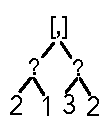
\includegraphics[scale=.25]{figures/tree1.pdf}

\noindent
At each choice point we can go either left or right, making such a decision
at each points leads to visit one particular tuple.

\hspace{-4mm}{\small
\begin{tabular}{@{}l@{~}ll@{~}ll@{~}ll@{~}l}
\begin{minipage}{1.2cm}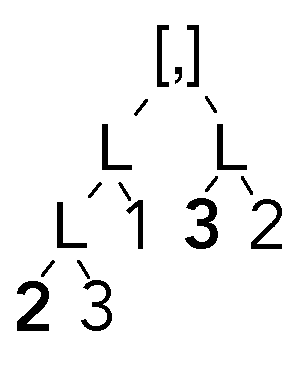
\includegraphics[scale=.25]{figures/tree2.pdf} 
\end{minipage} &  $ =   \tuple{p_2,p_3} $ &
\begin{minipage}{1.2cm}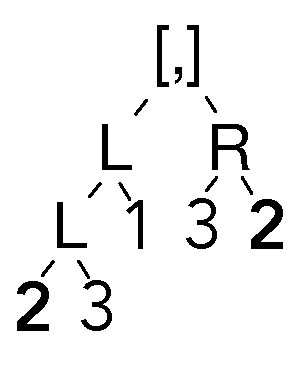
\includegraphics[scale=.25]{figures/tree3.pdf} 
\end{minipage} &  $ =   \tuple{p_2,p_2} $ 
&\begin{minipage}{1.2cm}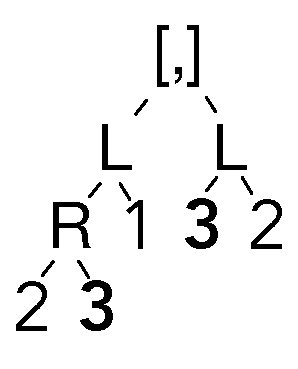
\includegraphics[scale=.25]{figures/tree4.pdf} 
\end{minipage} &  $ =   \tuple{p_2,p_3} $ \\
\begin{minipage}{1.2cm}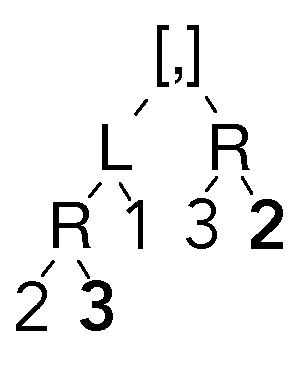
\includegraphics[scale=.25]{figures/tree5.pdf} 
\end{minipage} &  $ =   \tuple{p_2,p_2} $  &
\begin{minipage}{1.2cm}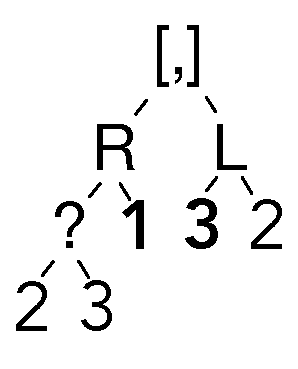
\includegraphics[scale=.25]{figures/tree6.pdf} 
\end{minipage} &  $ =   \tuple{p_3,p_2} $ 
&\begin{minipage}{1.2cm}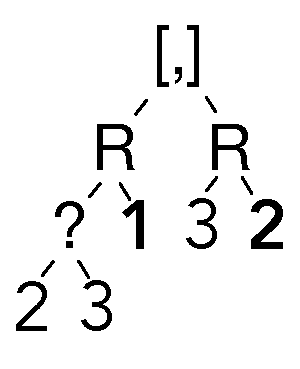
\includegraphics[scale=.25]{figures/tree7.pdf} 
\end{minipage} &  $ =   \tuple{p_3,p_3} $ 
\end{tabular}}

\noindent 
So, each tuple is uniquely determined from the original type term $t$ and a
choice string $c$. In the above example, iteration through the normalized,
union-free, type terms is defined by the sequence of choice strings \L\L\L,
\L\L\R, \L\R\L, \L\R\R, \R\L, \R\R. The length of the strings of choices is
bounded by the number of unions in a term.  The strings do not necessarily
have the same length.


The iteration sequence in the above example is thus \L\L\uL $\rightarrow$
\L\uL\R $\rightarrow$ \L\R\uL $\rightarrow$ \uL\R\R $\rightarrow$ \R\uL
$\rightarrow$ \R\R. Stepping from a choice string $c$ to next string
consists of splitting the string such that $c = c' \,\L\,c''$ and $c''$ is a
possibly empty sequence of \R.  The next string is $c'\, \R \, c_{pad}$,
that is to say it retain the prefix $c'$, toggles the \L to an \R and is
padded by a sequence of \L.  If there is no \L in $c$, iterations has
terminated.

Iteration is performed by calling the \c{next} function with a type term and
a choice string. \c{next} either returns the next string in the sequence or
\c{None}. Internally, it calls on \c{step} to toggle the last \L and shorten
the string (constructing $c'\,\R$). Then it call on \c{pad} to add the
trailing sequence of \L (constructing $c'\,\R\,c_{pad}$).

\begin{lstlisting}
type choice = L | R

let rec next(a:typ)(l:choice list) = 
  match step l with
   | None -> None
   | Some(l') -> fst (pad a l')
\end{lstlisting}

The \c{step} function delegates to \c{toggle} the job of flipping the last
occurrence of \L. For ease of programming, it reverses the choice string so
that \c{toggle} can be written as a simple recursion without an accumulator.
If the given choice string has no \L, then \c{toggle} returns empty, and
\c{step} returns \c{None}.

\begin{lstlisting}
let step (l:choice list) =
  match rev (toggle (rev l)) with
  | [] -> None
  | hd::tl -> Some(hd::tl)

let rec toggle = function
  | [] -> []    
  | L::tl -> R::tl
  | R::tl -> toggle tl
\end{lstlisting}

The \c{pad} function take a type term and a choice string to be padded. It
returns a pair, the first element is the padded string and the second is
remaining string. \c{pad} traverses the term, visiting both side of each
tuple, and for unions it uses the given choice string to direct its visit.
Each union encountered consumes a character out of the input string, once
the string is fully consumed, any remaining unions are treated as if there
was a \L. The first component of the returned value is the choice given as
argument extended with a number of \L corresponding to the number of unions
encountered after string ran out.

\begin{lstlisting}
let rec pad = function
   | (Prim i,l) -> ([],l)
   | (Tuple(t,t'),l) -> 
      let (h,tl) = pad t l in
      let (h',tl') = pad t' tl in (h @ h',tl')
   | (Union(t,_),L::r) -> 
      let (h,tl) = pad t r in (L::h,tl)
   | (Union(_,t),R::r) -> 
      let (h,tl) = pad t r in (R::h,tl)
   | (Union(t,_),[]) -> (L::(fst(pad t [])),[])
\end{lstlisting}

To obtain the initial choice string, the string only composed of \Ls, it
suffices to call \c{pad} with the type term under consideration and an empty
list. The first element of the returned tuple is the initial choice string. For
convienence, we will define the function \c{initial} for this purpose.

\begin{lstlisting}
let initial(t:typ) = fst (pad t [])
\end{lstlisting}


\subsection{Subtyping}

Subtyping visits union-free type terms using choice strings to iterate.  The
\c{subtype} function takes two type terms, \c a and \c b, and returns true
if they they are related by subtyping. It does this by iterating over all
union-free type terms in \c a, and checking that for each of them, there
exists a union-free type term in \c b that is a super-type.

\begin{lstlisting}
let subtype(a:typ)(b:typ) = allexists a b (initial a)
\end{lstlisting}

The \c{allexists} function take two type terms, \c a and \c b, and a choice
string \c f, and return true if \c a is a subtype of \c b for the position
in the iteration sequence specified by \c f. This is achieved by recursively
testing that for each union-free type term in \c a (induced by \c a and the
current value of \c f), there exists a union-free supertype in \c b.

\begin{lstlisting}
let rec allexists(a:typ)(b:typ)(f:choice list) =
  match exists a b f (initial b) with 
  | true -> (match next a f with
             | Some ns -> allexists a b ns 
             | None -> true) 
  | false -> false
\end{lstlisting}

Similarly, the \c{exists} function takes two type terms, \c a and \c b, and
two choice strings, \c f and \c e. It returns true if there exists in \c b a
union-free supertype of the type specified by \c f in \c a. This is done by
recursively iterating through \c e. The determination if two terms are
related is delegated to \c{sub}.

\begin{lstlisting}
type res = NotSub | IsSub of choice list * choice list

let rec exists(a:typ)(b:typ)(f:choice list)(e:choice list) =
 match sub a b f e with 
  | IsSub(_,_) -> true 
  | NotSub -> 
     (match next b e with
      | Some ns -> exists a b f ns 
      | None -> false) 
\end{lstlisting}

Finally, the \c{sub} function take two type terms and two choice strings and
return a value of type \c{res} which can be \c{NotSub} to indicate that the
types are not subtypes or \c{IsSub(_,_)} when they are.  If the two types
are primitives, then they are only subtypes if they are the same primitive
types.  If the two types are tuples, they are subtpyes is both of their
elements are subtypes. Not that the return type of \c{sub}, when successful,
hold the unused choice strings for both type term arguments. When confronted
with a union, \c{sub} will follow the choice string to decide which branch
to take. Consider for instance the case when the first type term is
\c{Union(t1,t2)} and the second is some type \c{t}, if the first element of
the choice string is an \L, then \c{t1} and \c{t} will be checked, otherwise
\c{sub} will check \c{t2} and \c{t}.

\begin{lstlisting}
let rec sub = function
 | (Prim i,Prim j,f,e) -> if i==j then IsSub(f,e) else NotSub
 | (Tuple(a1,a2), Tuple(b1,b2),f,e) ->
    (match sub a1 b1 f e with
     | IsSub(f', e') -> sub a2 b2 f' e'
     | NotSub -> NotSub)
 | (Union(a,_),b,L::f,e) -> sub a b f e
 | (Union(_,a),b,R::f,e) -> sub a b f e
 | (a,Union(b,_),f,L::e) -> sub a b f e
 | (a,Union(_,b),f,R::e) -> sub a b f e
\end{lstlisting}

\subsection{Further optimizations}

We have presented our subtyping algorithm using lists of choices. In a
practical implementation, however, these lists of choices can be efficiently
implemented (without allocation) by means of bit sets. This is the approach
taken in the Julia implementation of this algorithm. With this optimization,
the needed memory to decide a subtyping judgment is linear in the total number
of unions in the given types; the algorithm needs no allocation beyond that
of the choice stacks themselves.

\section{Correctness and completeness}

Our proof strategy for our algorithms broadly follows the above presentation.
We prove that iterators based on the intuition of making choices in the type
tree can be used to decide subtyping, then use this framework to prove the
choice string-based algorithm correct. We will focus on the core results,
while full details of the proof can be found in our complete Coq
mechanization.

In order to prove correctness of the subtyping algorithm, we must first establish
a definition for correctness. Guided by semantic subtyping and the normalization based
algorithm for subtyping, we define a denotational semantics for types that describes
compound types as sets of types without unions.

The denotational semantics we use for types is as follows:

\begin{align*}
\denotes{p_i} &= \{p_i\} \\
\denotes{\union{t_1}{t_2}} &= \denotes{t1} \cup \denotes{t2} \\
\denotes{\tuplet{t_1}{t_2}} &= \{\tuplet{t'_1}{t'_2} | t_1' \in \denotes{t_1},  t_2' \in \denotes{t_2'}\} \\
\end{align*}

Using this denotational semantics for types-with-unions, we can define
subtyping as if $\denotes{t_1} \subseteq \denotes{t_2}$, then $t_1 <: t_2$.
Equivalently, we can state this as definition~\ref{dfn:scr}, which is canonicalized
in our Coq proof as the \verb|NormalSubtype| relation.

\begin{definition}[Subtyping Correctness]
A subtyping relation $<:$ is correct if $t_1 <: t_2$ iff $\forall t_1' \in \denotes{t_1},
\exists t_2' \in \denotes{t_2}, t_1 <: t_2$.
\label{dfn:scr}
\end{definition}

Proving a subtyping algorithm sound and complete is therefore equivalent to
producing a function of type \verb|forall t1 t2:type, {NormalSubtype t1 t2} + {~NormalSubtype t1 t2}|; 
that is, the function is able to decide whether two types are
subtypes or not.

Subtyping with normalization is trivially complete in this framework; the
normalization procedure computes the full set of types denoted by each side
and then directly checks set inclusion.

However, what remains to be shown is that the iterator system is equivalent to
normalization. We do so by first proving that tree-based iterators, iterators
that assign choices to specific nodes within the type AST, iterate over the
list of base types that normalization produces. We then prove the same
property of list-based iterators by equivalence to tree-based iterators, and
conclude by proving that the three methods all can be used to decide subtyping
in a sound and complete manner.

\subsection{Iterators}

As described previously, we can use choices directly asigned to AST tree nodes
as our iterator state. We do so in Coq using so-called structural iterators,
which iterate over the structure of the type AST. By retaining the structure
in the iterator, we make it explicit which component of the type is having a
choice assigned to it. These iterators are defined as the following:

\begin{small}\begin{verbatim}
Inductive iter: type -> Set :=
| IPrim : forall i, iter (atom i)
| ITuple : forall t1 t2, iter t1 -> iter t2 -> iter (tuple t1 t2)
| IUnionL : forall t1 t2, iter t1 -> iter (union t1 t2)
| IUnionR : forall t1 t2, iter t2 -> iter (union t1 t2).
\end{verbatim}\end{small}

We can then define a stepping function for \verb|iter|s, which
steps a choice assignment on the tree to the next. We step depth-first,
left-to-right, so as to maintain the same order as we iterate through 
choice strings.

\begin{verbatim}
Fixpoint next_tree (t:type)(ti:iter t) : option (iter t) :=
  match ti with
  | IPrim i => None
  | ITuple2 ti1 ti2 p1 p2 =>
    match (next_tree ti2 p2) with
    | Some (np2) => Some(ITuple2 ti1 ti2 p1 np2)
    | None =>
      match (next_tree ti1 p1) with
      | Some (np1) => Some(ITuple2 ti1 ti2 np1 (start_iterator ti2))
      | None => None
      end
    end
  | IUnionL ti1 ti2 pl =>
    match (next_tree ti1 pl) with
    | Some(npl) => Some(IUnionL ti1 ti2 npl)
    | None => Some(IUnionR ti1 ti2 (start_iterator ti2))
    end
  | IUnionR ti1 ti2 pr => option_map (TIUnionR ti1 ti2) (next_tree ti2 pr)
  end.
\end{verbatim}

We have four cases to worry about. If given a primitive type, there is no
successor state. A tuple will first attempt to step its second child; if  that
has no successor step, then it will step its first child and reset the second
child (the truncate operation, but for trees). When given a union which goes
left, it will check if the left branch has a state remaining and take it if
possible. Otherwise, it will step to take the right branch on the union and
re-initialize the iterator for the right branch. \verb|next_tree| returns
\verb|Some s| if there is some successor state \verb|s| to the current, and
\verb|None| if the given iterator state is terminal.

TODO: figure.

We can now define an induction principle over \verb|next_tree|. It is guaranteed
to eventually reach a state from which it cannot step (as it forever moves right
through the type tree). 

\begin{theorem}
\begin{small}\begin{verbatim}
Definition iter_rect
  (t:type) (P:iter t -> Set)
           (pi: forall it, next_tree t it = None -> P it)
           (ps : forall it' it'', P it'' -> next_tree t it' = Some it'' -> P it')
           (it : iter t) : P it  
\end{verbatim}\end{small}

For any type \verb|t| and proposition \verb|P|, and if:
\begin{itemize} 
	\item \verb|P| holds for an iterator that has no next state (e.g. is done)
	\item if \verb|P| holds for the \emph{following} iterator state \verb|it|,
	then \verb|P| holds for the \emph{preceding} iterator state \verb|it'|.
\end{itemize}
Then \verb|P| holds for all iterators for type \verb|t|
\end{theorem}
\begin{proof}
We can compute the number of steps remaining in an iterator given its present state
and the type over which it is iterating (see the \verb|iternum| function in Coq for
details). As \verb|next_tree| steps, the value of \verb|iternum| monotonically decreases.
As a concequence, we can use induction over the naturals on \verb|iternum| as the basis
for our induction hypothesis for tree iterators.

If \verb|iternum| is 0, then it follows that \verb|next_tree| cannot take a step. Therefore,
\verb|pi| applies and the theorem holds.

If \verb|iternum| is \verb|S n| for some \verb|n|, then \verb|next_tree| can take a step to a state for which
\verb|iternum = n|. By the IH, we can assume that \verb|P| holds for states in which \verb|iternum = n|, 
and therefore we can apply \verb|ps| and the theorem holds.

For full details, see the Coq definition of \verb|iter_rect|.
\end{proof}

Using \verb|iter_rect|, we can implement and prove correct equivalent functions
to \verb|exists|, and \verb|allexists|. Therefore, we can prove a version of \verb|subtype|
based on iteration over choice trees.
\begin{small}\begin{verbatim}
Definition exists_iter(a b : type) : 
  ({ t | InType t b /\ BaseSubtype a t } +
   {forall t, InType t b -> ~(BaseSubtype a t) }).
\end{verbatim}\end{small}

\verb|exists_iter| is equivalent to the choice-stack based \verb|exists|,
and determines if there exists some denotationally-contained type in \verb|b|
that is a supertype of the given \verb|a|. Internally, it is implemented in 
the same way as \verb|exists|, though using \verb|iter_rect| to iterate 
through every iterator state.

\begin{small}\begin{verbatim}
Definition forall_iter (a b : type) :
  { forall t, In t (clauses a) -> exists t', InType t' b /\ (BaseSubtype t t')} +
  { exists t, In t (clauses a) /\ forall t', InType t' b -> ~ (BaseSubtype t t')}.
\end{verbatim}\end{small}

\verb|forall_iter| is to \verb|allexists| what \verb|exists_iter| is to
\verb|exists|. Like \verb|exists_iter| it implements the same decision procedure
as \verb|allexists| (and internally relies upon \verb|exists_iter|), though through
the abstraction of \verb|iter_rect|.

Finally, we can define a decidable function (called \verb|subtype| in the proof)
that decides whether two types are subtypes or not. \verb|subtype| simply invokes
\verb|forall_iter| to decide subtyping.

\begin{small}\begin{verbatim}
Definition subtype(a b:type) : {NormalSubtype a b} + {~NormalSubtype a b}.
  destruct (forall_iter a b).
  - left. [...]
  - right. [...]
Defined.
\end{verbatim}\end{small}

\noindent Therefore, using iterators, we can decide whether subtyping holds for any two types
in our language. We will now show an equivalence between iterators and stacks-of-choices,
allowing for more efficient implementation.

\subsection{Stacks}

To show that the choice-stack based algorithm is correct, we reduce it to the
already-shown-correct iterator-based algorithm for deciding subtyping. To do so,
we show an equivalence between choice stacks and iterators, then prove correctness
of the subtyping algorithms.

In the context of the Coq proof, we use the type \verb|st_context| to refer
to a choice stack. In Coq, this is represented as a list of boolean values,
with false representing a left choice and true representing a right choice at
a specific union.

To show equivalence between the iterator-based and stack-based algorithm, we need to
first prove two properties:

\begin{itemize}
  \item iterators are convertible to equivalent choice lists;
  \item stepping an iterator is equivalent to stepping a choice list.
\end{itemize}

We define an iterator and a choice stack to be equivalent if, when applied to
the same type, they select the same subset of that type. To describe this, we
define \verb|lookup_path| which looks up what type is selected by a given
choice stack.

\begin{small}\begin{verbatim}
Fixpoint lookup_path(t:type)(p:st_context) : type * st_context :=
  match t, p with
  | atom i, _ => (t, p)
  | tuple t1 t2, _ =>
    let (r1,p1) := lookup_path t1 p in
    let (r2,p2) := lookup_path t2 p1 in
    (tuple r1 r2, p2)
  | union l r, false::rs => lookup_path l rs
  | union l r, true::rs => lookup_path r rs
  | _, nil => (t, nil)
  end.
\end{verbatim}\end{small}

\verb|lookup_path| is notable in that it both returns the selected type as
well as whatever of the choice stack remains once it reaches a leaf. This is
needed in order to be able to traverse types that contain tuples,  whose left
branches will potentially be given a longer choice stack then necessary.

Next, we can convert iterators to paths in the straightforward manner, as
implemented by \verb|iterator_to_path|:

\begin{small}\begin{verbatim}
Fixpoint iterator_to_path(t:type)(it:TypeIterator t):st_context :=
   match it with
   | TIPrim _ => nil
   | TITuple t1 t2 it1 it2 => (iterator_to_path t1 it1) ++ (iterator_to_path t2 it2)
   | TIUnionL t1 _ it1 => false :: (iterator_to_path t1 it1)
   | TIUnionR _ t2 it1 => true :: (iterator_to_path t2 it1)
   end.
\end{verbatim}\end{small}

\verb|iterator_to_path| simply traverses the iterator in order, appending onto the
output choice stack whatever choice the iterator makes at that union. This illustrates
the equivalence between iterators and choice stacks; choice stacks are simply iterators
with the structural information removed.

Using the combination of \verb|lookup_path| and \verb|iterator_to_path|, we
can then show the first correctness property that we need to prove that the
algorithm using choice stacks is correct:

\begin{lemma}[Iterator to path is correct]
\begin{small}\begin{verbatim}
Lemma itp_correct : forall t it, 
  current t it = fst (lookup_path t (iterator_to_path t it)).
\end{verbatim}\end{small}

For every type \verb|t| and type iterator \verb|it|, the iterator's current type \verb|current t it| is equal
to the result of looking up the conversion of \verb|it| to a choice stack.
\end{lemma}
\begin{proof}
See \verb|itp_correct| in the Coq proof.
\end{proof}

Stepping in the Coq implementation is implemented identically to the OCaml
implementation. It only remains to show that this step operation (called
\verb|step_ctx| in Coq) is correct with respect to the iterator
\verb|next|.

\begin{lemma}[Correctness of step\_ctx]
\begin{small}\begin{verbatim}
forall t it,
    step_ctx t (iterator_to_path t it) =
    (option_map (iterator_to_path t) (next t it)).
\end{verbatim}\end{small}
For every type \verb|t| and type iterator \verb|it|,
stepping the choice-list equivalent of \verb|it| will
produce the same result as converting the result of stepping
\verb|it|.
\end{lemma}
\begin{proof}
See \verb|list_step_correct| in the Coq proof.
\end{proof}

Now, with the relevant properties proven, we can implement and prove correct
\verb|exists| and \verb|allexists| in Coq. The function names are the
same, as are the implementations up to the addition of a fuel parameter (which
is shown to be unnecessary). 

\begin{lemma}[Correctness of existential subtype checking with choice stacks]
\begin{small}\begin{verbatim}
forall a b it, 
  (exists pf, exists_iter_inner a b it = inleft pf) <->
   exists n, exists a b (iterator_to_path b it) n = Some true.
\end{verbatim}\end{small}
For every two types \verb|a| and \verb|b|, the iterator-based algorithm
\verb|exists_iter_inner| will produce a proof that \verb|a| is a subtype
of \verb|b| if and only if there is an integer \verb|n| such that
 \verb|exists| given \verb|n| fuel runs producing true.
\end{lemma}
\begin{proof}
See \verb|ex_sub_corr_eq| in the Coq proof.
\end{proof}

\begin{lemma}[Correctness of forall-exists subtype checking with choice stacks]
\begin{small}\begin{verbatim}
forall a b it,
   (exists pf, forall_iter_inner a b it = left pf) <->
    exists n, allexists a b (iterator_to_path a it) n = Some true.
\end{verbatim}
\end{small}  
For every two types \verb|a| and \verb|b|, the iterator-based algorithm
\verb|forall_iter_inner| will produce a proof that \verb|a| is a subtype
of \verb|b| if and only if there is an integer \verb|n| such that
 \verb|allexists| given \verb|n| fuel runs producing true.
\end{lemma}
\begin{proof}
See \verb|fa_sub_corr_eq| in the Coq proof.
\end{proof}

The choice stack-based algorithm therefore is provably equivalent to the
iterator-based algorithm, and is thus correct.

\section{Performance Analysis}

The algorithm improves upon normalization in two key ways:
\begin{itemize}
  \item lazily exploring possible clauses, obviating the need to store a
    fully normalized type;
  \item enabling fast paths that avoid the exploration of the full choice space.
\end{itemize}

\noindent
In the worst case, our algorithm has the same big-O time complexity as
normalization. However, lazily exploring the choice space allows us to
require worst-case polynomial space, in comparison to normalization's
exponential space complexity.  Similarly, the algorithm enables
optimizations that offer best (and typical) case time complexity
improvements from exponential to linear time.

Worst case time complexity of both subtyping algorithms is determined by the
number of clauses that would exist in the normalized type. In the worst case,
(a tuple of unions), each union begets a different clause in the normalized
type. Consider $\tuple{\union{A}{B}, \union{C}{D}}$, which will normalize to
$\union{\tuple{A,C}}{\tuple{A, D}, \tuple{B, C}, \tuple{B, D}}$ generating a 
new tuple for each choice for every contained union. As a result, there are
worst-case $2^n$ tuples in the fully normalized version of a type that has $n$
unions.

In order to ensure correctness, each of these tuples (or choices at unions)
must always be explored. As a result, both the algorithm we present here and
normalization will have worst-case $O(2^n)$ time complexity. The approaches
differ, however, in space complexity. The normalization approach computes and
stores each of the exponentially many alternatives, so also has $O(2^n)$ space
complexity. However, the algorithm we discuss need only store the choice made
at each union, thereby offering $O(n)$ space complexity.

The algorithm we discuss also can improve best-case time performance.
Normalization will necessarily be $o(2^n)$ due to computation of the entire
normalized type. However, the lazy subtyping algorithm need only make one
choice before discovering that a subtype relation exists in the best-case,
giving $o(n)$ performance. Moreover, computing type choices lazily enables
fast-paths to short circuit full exploration of choice alternatives.

This is important for Julia due to a common programming idiom. Many Julia
library developers write signatures of the form $\tuple{\union{A}{B},
\union{C}{D}}$ to indicate that their method can take any of the named
types. When deciding dispatch against these methods, Julia will frequently
check if a tuple containing solely concrete (instantiable) types is a subtype 
of the tuple of unions. If Julia used normalization, this would always be 
exponential on the number of unions that appeared in the argument list as this
is the above mentioned worst-case exponential complexity case. However, its use
of the lazy algorithm enables it frequently identify the best alternative and
short circuit before having to explore much of the choice possibility space.

\section{Conclusion}

We have presented an algorithm for deciding subtyping relationships between
types that consist of atomic types, tuples, and unions. This algorithm is able
to decide subtyping relationships in the presence of distributive semantics
for union types without needing normalization (and therefore using linear
space) and without additionally constraining type system features.

\subsubsection*{Acknowledgments}
The authors thank Jiahao Chen for starting us down the path of understanding
Julia, and Jeff Bezanson for coming up with Julia's subtyping algorithm.  This
work received funding from the European Research Council under the European
Union's Horizon 2020 research and innovation programme (grant agreement
695412), the NSF (award 1544542 and award 1518844) and the Czech Ministry of
Education, Youth and Sports (grant agreement
CZ.02.1.01/0.0/0.0/15\_003/0000421).
 

%\bibliographystyle{plain}
\bibliography{refs}
\end{document}
